\chapter{Dark matter}
\label{ch:dm}
%P1, the Standard Model -> dark matter
\par As mentioned in Chapter~\ref{ch:sm}, about one quarter of the total mass-energy in the universe is dark matter. No known particle that can account for the dark matter in the universe, and single-particle model is disfavored. Therefore, current models consider dark matter as a whole sector of new particles, instead of the existence of a single new type of particle.

%P2, chapter structure
\par This chapter is organized as follows: the astrophysical measurements establishing of dark matter and its particle physics explanation are discussed in Section~\ref{sec:dms1}. In Section~\ref{sec:dms2}, dark matter as a microscopic particle, Weakly Interacting Massive Particle, is described. Finally, Section~\ref{sec:dms3} outlines how dark matter particles might be produced by particle colliders and what signatures they might generate.

\section{The dark matter: From astrophysics to particle physics}
\label{sec:dms1}

%P1,
\par The concept of dark matter originates from physical observations. Multiple astrophysical observations at different distance scales prove the existence of invisible matter in the universe. The dark matter concept was formally brought up by Jacobus Kapteyn in the studies of the velocity distribution of stars in nearby galaxies\cite{Kapteyn:1922zz}. These studies showed that the amount of visible matter from stars and interstellar gas near the solar system was not sufficient to explain the motions of the stars perpendicular to the Milky Way disk. The visible matter doesn't provide enough gravitational force attraction which suggests the existence of the unobserved matter. Another proof on galactic scales is the motion of the Coma galaxy cluster observations by Fritz Zwicky in 1933\cite{Zwicky:1933gu}, which suggested a large contribution to the gravitational forces that is not visible.

\par On galactic scales, the most convincing evidence is the direct observation of the rotation curves of galaxies, which shows the orbital velocities of stars and gas inside a galaxy as a function of their distance from the galactic center. According to the Newtonian theory of gravity, the rotation velocity, $v(r) \propto \frac{1}{\sqrt{r}}$, which is in contrast with observed curve in Fig~\ref{fig:rotation}. It is the discrepancy between the observed and expected velocities that has led to the belief that some form of dark matter must exist. And this suggests the existence of a dark (invisible) halo with $M(r) \propto r$ and $\rho \propto \frac{1}{r^2}$.

\begin{figure}[htbp]
  \begin{center}
    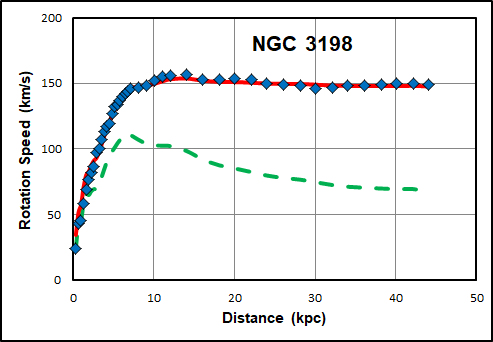
\includegraphics[width=0.8\textwidth]{chapters/c2/figures/ngc3198_sparc.jpg}
  \end{center}
  \caption{The rotation curve for spiral galaxy NGC 3198. The blue diamonds are the observations and reveal the almost flat-like nature of the curve in the outer regions of the galaxy. The dashed green line is the curve for Newtonian gravity. It shows that the rotational velocity should decrease with distance from the galaxy center. The solid red line through the data points is the curve obtained by assuming a simple Gaussian energy scale variation and a simple Gaussian density distribution for the galaxy.}
  \label{fig:rotation}
\end{figure}

\par The Cosmic Microwave Background (CMB), is electromagnetic radiation remnant from an early stage of the universe, also known as ``relic radiation''. On the cosmological scale, not only does CMB show evidence of dark matter, in the context of specfic models it also quantifies the amount of dark matter in the Universe. Experiments measure the power spectrum of the CMB. Now the Lambda-CDM model best fits the observation data, giving values for the density of baryonic matter, dark matter, and Dark Energy.

\par Hot dark matter (HDM) theory\cite{Zeldovich:1982zz} was established in 1980 by Zeldovich's team. HDM assumes that the light neutrinos make up the majority of the dark matter. It is natural to assume that the dark matter is the weakly coupled particle that already exists in the Standard Model. However, the conventional neutrino-dominated picture is ruled out by early universe simulation studies in 1983\cite{White:1984yj}. Afterwards, scientists realized that only with a slow-paced particle, so-called ``cold'' dark matter, the diffusion of small scale fluctuation can be prevented. The early universe structure can be formed on all scales is consistent with this astrophysical observations. Therefore, the cold dark matter theory (CDM theory)\cite{PhysRevLett.48.223} was established in 1983 to explain the cosmic microwave background observation result. Nowadays, as an important part of the standard cosmological model (Lambda-CDM theory), the concept of cold dark matter is widely accepted. 

\section{Weakly Interacting Massive Particles}
\label{sec:dms2}
%P1, why WIMPs
\par Although the existence of cold dark matter around galaxies and clusters is supported by cosmological observation, scientists still have no clue about what exactly the cold dark matter is. Based on the reductionism, the observation of cold dark matter indicates the existence of weakly interacting fundamental particles. And since the density fluctuation is derived by the cold dark matter candidate mass, and the small scale fluctuation is not supposed to be dissolved, the mass of cold dark matter candidate can not be light. Therefore, the WIMPs - weakly interacting massive particles becomes one of the best candidate particles that characterize the feature of cold dark matter.

%P2, WIMPs in beyond the Standard Models
\par the mass of WIMPs are range from a few GeVs to $\mathcal{O}$(TeV), which matches observed relic density from CMB analysis. Both in the two popular beyond SM models Supersymmetry (SUSY) and Extra-dimensions, there are WIMP candidates of DM particles. The electrically neutral lightest supersymmetric particle (LSP) predicted in an R-parity conserved scenario of minimal supersymmetric extension of the Standard Model (MSSM) is an ideal candidates of dark matter. Among all possible choices, the most promising one is the lightest neutralino, which is the lightest state of mixtures of neutral electroweak gauginos and the neutral higgsinos\cite{Feng:2010gw}. Similar to the phenomenology of the MSSM, in minimal universal extra dimensions (MUED) model, each SM particle is accompanied by a partner particle at the first Kaluza-Klein (KK) mode level. Also, the MUED model possesses a geometric parity (KK parity). The lightest partner state (which in MUED is the partner of the $U(1)_Y$ gauge boson) represents dark matter candidate which matches the observed dark matter relic density\cite{Servant:2002aq}.

\section{Search dark matter in collider experiment}
\label{sec:dms3}
%P1, experimental method to search dark matter
\par dark matter was observed through its gravitational interaction in galaxies. To explore its further particle properties, several complementary detection methods are used as showed in \cite{Undagoitia:2015gya}: 
\begin{itemize}
  \item \textbf{Direct detection}: The direct detection is focus on recoils of nuclei with few keVs that induced by interactions with dark matter particle candidate.
  \item \textbf{Indirect detection}: The indirect detection is searching the dark matter signals from annihilation products, usually in cosmic rays.
  \item \textbf{Production at colliders}: The production at colliders, as its name suggest, looking for WIMPs in collision data. WIMPs can be detected indirectly as missing energy and momentum that escape the detectors, assume that all other collision products are detected as negligible interactions with normal visible matter.
\end{itemize}

%P2, search dark matter in collider experiment
\par In the rest of this thesis, only the ``Production at collider'' approach will be described. Several beyond the Standard Models that have dark matter candidate will be described in the rest of this section. These models are the search target and will be interpreted in statistical manner with collision data.

\subsection{Effective field theory}
%P1, why EFT
Before we dive into the specific particle physics model, some generic principals need to be illustrated. The first concept is the effective field theory. The effective field theory is a type of approximation for an underlying physical theory, for example, quantum field theory. According to reductionism, all physical observations need to be explainable with one single physics theory. However, since this “theory of everything” is supposed to explain the experiment at all energy scales, the physical observables are always resulted in infinite under the quantum field theory framework. Furthermore, the important features of the known physics, namely the Standard Model, are not guaranteed to be extendable with higher energy scale. Therefore, the ultraviolet energy cut-off is needed for quantum field theory based particle physics model to guarantee the model itself renormalizable. The effective field theory\cite{Pich:1998xt} is designed to resolve this issue.

%P2, what is EFT
\begin{figure}[htbp]
  \begin{center}
    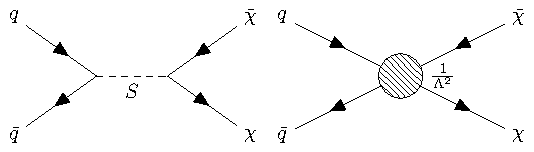
\includegraphics[width=0.8\textwidth]{chapters/c2/figures/eft-feyn-diagram}
  \end{center}
  \caption{Left: an s-channel Feynman diagram of the interaction between quarks and dark matter candidates via a scalar mediator; Right: the corresponding effective field theory contact interaction.}
  \label{fig:c2eftfeyndiagram}
\end{figure}

In the context of particle physics, the effective field theory are simplifications of the complete quantum field theories where the mass of interaction mediator is large enough with respect to the momentum exchange of a physical process. Therefore, the s-channel process can be replaced by a contact operator as demonstrated in Fig~\ref{fig:c2eftfeyndiagram}. In Fig~\ref{fig:c2eftfeyndiagram}, a new scalar mediator, labeled as S, is introduced to couple with both the Standard Model quarks and dark matter candidate. The Lagrangian of this simple model is listed in the following Equation~\ref{eq:c2eftl}:

\begin{equation}
  L = \frac{1}{2}M^{2}S^{2}-g_{q}q\bar{q}S-g_{\chi}\chi\bar{\chi}S,
  \label{eq:c2eftl}
\end{equation}

where M is the mass of newly introduced scalar, $g_{\chi}$ is the coupling strength between the scalar mediators and dark matter candidates, and $g_{q}$ is the coupling constant between the scalar mediators and the Standard Model quarks. The knowledge of the quantum field theory tells us that the s-channel cross section is proportional to the factor $\frac{1}{Q_{tr}^{2}-M^{2}}$, where $Q_{tr}$ is the momentum transfer of the process. Using Taylor expansion, this factor can be expanded in powers of $\frac{Q_{tr}}{M}$: 

\begin{equation}
  L = \frac{1}{2}M^{2}S^{2}-g_{q}q\bar{q}S-g_{\chi}\chi\bar{\chi}S
  \label{eq:c2taylorexp}
\end{equation}

If $Q_{tr} \ll M$, the propagator term can be simplified as $-\frac{1}{M^2}$. Therefore, the interaction vertices of s-channel collapsed into a contact point in a contact point: $O_{s}=\frac{g_{q}g_{\chi}}{M^{2}}\chi\bar{\chi}q\bar{q}$, where $\Lambda=\frac{g_{q}g_{\chi}}{M^{2}}$ can be viewed as the mass scale of the effective field theory. Given the condition that $Q_{tr} \ll M$, the constraint of the new energy scale can be derived as equation~\ref{eq:c2scalelimit}:

\begin{equation}
  \Lambda \gg \frac{Q_{tr}}{\sqrt{g_{q}g_{\chi}}}
  \label{eq:c2scalelimit}
\end{equation}

Therefore, the simulation calculation can be simplified for any process that satisfies the condition~\ref{eq:c2scalelimit}.

\subsection{The simplified model}
%P1, why simplified model
\par Although the energy scale can be limited with the effective field theory, the simulation can still be complex due to the model structure itself. For example, in the simplest scenario of the supersymmetry model, the Minimal Supersymmetric Standard Model, more than 100 parameters needed to be determined. It is almost impossible for experimentalist to explore them all together within a search for one signature. Therefore, the idea of simplified model\cite{SimplifiedModels-Alves2012} is here to rescue.

%P2, what is simplified model
\par A simplified model describes the interaction mediator that couples with the Standard Model particle and new particle that defined in the model beyond the Standard Model. With the help of simplified model, the complex interaction Feynnman diagram group can be simplified trimmed into one or several tree-level diagrams that described the signal of interest. As a result, the model simulation calculation is simplified while the model characteristics are still preserved. 

%P3
\par With the simplification of effective field theory and simplified model, several models are introduced in the rest of this section. The physical events from these models are served as search signal for the rest of the thesis.

\subsection{$Z^{\prime}$ model and Two-Higgs-doublet model}
%P1, Z' model, why
\par $Z^{\prime}$ model\cite{He:1991qd} is one of the simplest the Standard Model extensions that have dark matter candidate. As mentioned in the section~\ref{sec:dms2}, the ideal dark matter candidate as fundamental particle needs to be both weakly interacting and massive. Therefore, a natural way to introduce a weakly coupled particle into the Standard Model is to add a new vector boson that coupled with WIMPs. This newly added particle is a massive, neutral boson. The simplest gauge structure of this beyond the Standard Model is a U(1) extension with the Standard Model gauge. However, this newly added U(1) gauge can be a derivative from more complex symmetry, like SU(2), or $E_{6}$. This simplest extension of the Standard Model is called $Z^{\prime}$ model.

%P2, Z' model, what
\par The $Z^\prime$ particle can be coupled with both the Standard Model quarks and dark matter candidates. A typical Feynnman diagram is shown in the Fig~\ref{fig:c2zprime}. However, the mass of the dark matter candidate is highly constrained by the Higgs boson mass, therefore, it is less possible to find a massive dark matter candidate within the current experiment constraints in $Z^{\prime}$ model. But we can still mixing the $Z^{\prime}$ model with other beyond the Standard Models to gain more room in parameters phase space. One of the examples is $Z^{\prime}-2HDM$ model, a mixture of $Z^{\prime}$ model and Two-Higgs-doublet model.

%P3, 2HDM, why
\par Before describing the mixture model, let us mention the Two-Higgs-doublet model\cite{Branco:2011iw}, abbreviated as 2HDM. 2HDM is a multiple Higgs boson scenario extension of the Standard Model. The 2HDM model is inspired by the supersymmetry model\cite{Martin:1997ns} and the Axion model\cite{Peccei:2006as}. Therefore, the 2HDM can not only provide the dark matter candidate, but also brings enough CP violation space to support baryon asymmetry for early stage universe.

%TODO, P4, 2HDM, what, too many equations...

%P5, Z'+2HDM
\par As mentioned in the previous paragraphs, $Z^{\prime}$ model and Two-Higgs-doublet model can be combined into a mixture model to provide much richer phenomenological predictions. The Higgs-liked field in the 2HDM is introduced into $Z^{\prime}$ model as dark matter candidates’ mediator. As a result, the mixture $Z^{\prime}+2HDM$ model\cite{Berlin:2014cfa} can provide massive enough dark model candidate under experimental data constraint with its larger parameters space.

%P6, Higgs bb channel in 2HDM and Z'+2HDM
\begin{figure}[htbp]
  \begin{center}
    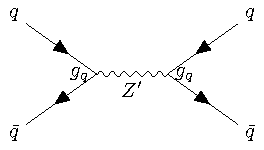
\includegraphics[width=0.5\textwidth]{chapters/c2/figures/z-prime}
  \end{center}
  \caption{The Feynman diagram of the interaction between the Standard Model quarks and $Z^{\prime}$ boson.}
  \label{fig:c2zprime}
\end{figure}

\begin{figure}[htbp]
  \begin{center}
    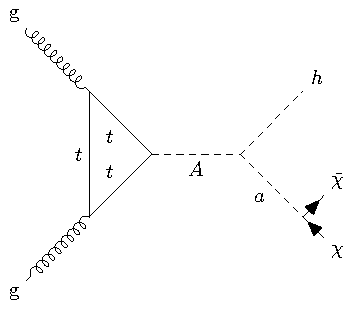
\includegraphics[width=0.5\textwidth]{chapters/c2/figures/two-higgs}
  \end{center}
  \caption{The Feynman diagram of the interaction between the Standard Model quarks and $Z^{\prime}$ boson.}
  \label{fig:twohiggs}
\end{figure}

\begin{figure}[htbp]
  \begin{center}
    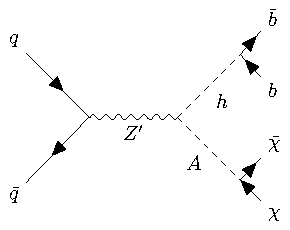
\includegraphics[width=0.5\textwidth]{chapters/c2/figures/z-prime-2hdm}
  \end{center}
  \caption{The Feynman diagram of $b\bar{b}$ decayed Higgs channel in $Z^{\prime}+2HDM$.}
  \label{fig:c2zprime2hdm}
\end{figure}


\par With the discovery of the Higgs boson, the study of Higgs properties becomes the frontier of particle physics. The Higgs tagging is also widely used as the new taggable physics object, like top quark after 1995, in the new physics search. The dark matter search with collider experiment also benefits from the newly discovered Higgs boson. The decay channels that have Higgs boson in the final state now ready for physicists to probe. Therefore, both the Two-Higgs-doublet model and $Z^{\prime}+2HDM$ can be explored with Higgs boson tagging. Among all the Higgs decay channels, the Higgs to $b\bar{b}$ is the one with the largest branching ratio. Therefore, it is natural for experimentalists to search the dark matter candidate with Higgs to $b\bar{b}$ decay as its signature. The Feynman diagram of $Higgs b\bar{b}$ channel is shown in Fig~\ref{fig:twohiggs} for Two-Higgs-doublet model, while in Fig~\ref{fig:c2zprime2hdm} for $Z^{\prime}+2HDM$. Both of them are studied as the signal in the rest of the thesis.
